\documentclass[a4paper,12pt]{report}

% --- Encoding & Font ---
\usepackage[utf8]{inputenc}
\usepackage[T5,T1]{fontenc}
\usepackage[english,vietnamese]{babel}
\usepackage{times}
\usepackage{lmodern}

% --- Page Layout ---
\usepackage[top=2.5cm, bottom=2.5cm, left=3cm, right=2.5cm]{geometry}
\usepackage{setspace}
\onehalfspacing

% --- Graphics ---
\usepackage{graphicx}
\usepackage{float}
\usepackage{subcaption}

% Pandoc image scaling & placement
\makeatletter
\def\maxwidth{\ifdim\Gin@nat@width>\linewidth\linewidth\else\Gin@nat@width\fi}
\def\maxheight{\ifdim\Gin@nat@height>\textheight\textheight\else\Gin@nat@height\fi}
\makeatother
\setkeys{Gin}{width=\maxwidth,height=\maxheight,keepaspectratio}
\makeatletter
\def\fps@figure{htbp}
\makeatother

% --- Tables ---
\usepackage{booktabs}
\usepackage{array}
\usepackage{longtable}
\usepackage{multirow}
\usepackage{tabularx}
\usepackage{calc}

% --- Math ---
\usepackage{amsmath}
\usepackage{amssymb}

% --- Code Listings & Verbatim with UTF-8 support ---
\usepackage{listings}
\usepackage{xcolor}
\usepackage{fancyvrb}
\usepackage{fvextra}

\definecolor{codebg}{RGB}{248,248,248}
\definecolor{codeframe}{RGB}{200,200,200}
\definecolor{codecomment}{RGB}{106,153,85}
\definecolor{codestring}{RGB}{163,21,21}
\definecolor{codekeyword}{RGB}{0,0,255}
\definecolor{ptitblue}{RGB}{0,51,153}

\lstdefinestyle{customstyle}{
  backgroundcolor=\color{codebg},
  frame=single,
  rulecolor=\color{codeframe},
  basicstyle=\ttfamily\footnotesize,
  keywordstyle=\color{codekeyword}\bfseries,
  commentstyle=\color{codecomment}\itshape,
  stringstyle=\color{codestring},
  showstringspaces=false,
  breaklines=true,
  tabsize=4,
  captionpos=b,
}
\lstset{style=customstyle}

\DefineVerbatimEnvironment{lstlisting}{Verbatim}{
  frame=single,
  rulecolor=\color{codeframe},
  fillcolor=\color{codebg},
  framesep=3mm,
  fontsize=\footnotesize,
  breaklines=true
}

% --- Hyperlinks ---
\usepackage[hidelinks]{hyperref}
\usepackage{url}
\usepackage{xurl}

% --- Section Formatting ---
\usepackage{titlesec}
\usepackage[titles]{tocloft}

% --- Compact TOC configuration to guarantee single-page fit ---
\setlength{\cftbeforetoctitleskip}{-15pt}
\setlength{\cftaftertoctitleskip}{15pt}
\setlength{\cftbeforechapskip}{4pt}
\setlength{\cftbeforesecskip}{1pt}

\titleformat{\chapter}[display]
  {\normalfont\fontsize{22}{26}\bfseries}
  {Chương \thechapter}{14pt}{\fontsize{22}{26}\bfseries}
\titlespacing*{\chapter}{0pt}{-10pt}{24pt}

\titleformat{\section}
  {\normalfont\fontsize{16}{20}\bfseries}{\thesection}{1em}{}
\titlespacing*{\section}{0pt}{18pt}{10pt}

\titleformat{\subsection}
  {\normalfont\fontsize{13}{17}\bfseries}{\thesubsection}{1em}{}
\titlespacing*{\subsection}{0pt}{14pt}{8pt}

\titleformat{\subsubsection}
  {\normalfont\fontsize{12}{15}\bfseries\itshape}{\thesubsubsection}{1em}{}
\titlespacing*{\subsubsection}{0pt}{10pt}{6pt}

% --- Caption ---
\usepackage{caption}
\captionsetup{font=small, labelfont=bf, skip=8pt}

% --- Header / Footer ---
\usepackage{fancyhdr}
\pagestyle{fancy}
\fancyhf{}
\fancyfoot[C]{\thepage}
\renewcommand{\headrulewidth}{0pt}

% --- TOC depth ---
\setcounter{tocdepth}{3}
\setcounter{secnumdepth}{3}

% --- Indentation ---
\usepackage{indentfirst}
\setlength{\parindent}{1cm}

% --- TikZ for cover page decorations ---
\usepackage{tikz}
\usetikzlibrary{calc}

% --- Pandoc compatibility macros ---
\providecommand{\tightlist}{%
  \setlength{\itemsep}{0pt}\setlength{\parskip}{0pt}}
\newcommand{\passthrough}[1]{#1}
\newcounter{none}

\begin{document}

% =============================================================
% TITLE PAGE
% =============================================================
\begin{titlepage}
\thispagestyle{empty}

% --- Decorative double-line border with corner ornaments ---
\begin{tikzpicture}[remember picture, overlay]
  % Outer border
  \draw[line width=1.6pt]
    ([shift={(1.2cm,-1.2cm)}]current page.north west)
    rectangle
    ([shift={(-1.2cm,1.2cm)}]current page.south east);
  % Inner border
  \draw[line width=0.5pt]
    ([shift={(1.45cm,-1.45cm)}]current page.north west)
    rectangle
    ([shift={(-1.45cm,1.45cm)}]current page.south east);
\end{tikzpicture}

\begin{center}

% --- University & Department header ---
\textbf{\fontsize{13}{16}\selectfont HỌC VIỆN CÔNG NGHỆ BƯU CHÍNH VIỄN THÔNG}\\[0.25cm]
\textbf{\fontsize{13}{16}\selectfont KHOA CÔNG NGHỆ THÔNG TIN 1}\\[0.15cm]

% --- Dashed separator ---
{\centering\rule[0.5ex]{10cm}{0.4pt}\par}

\vspace{0.8cm}

% --- PTIT Logo ---

\includegraphics[width=3.5cm]{logo.jpg}

\vspace{0.8cm}

% --- Subject title ---
{\fontsize{20}{26}\selectfont\bfseries\color{ptitblue}
BÁO CÁO CÀI ĐẶT HỆ THỐNG}\\[0.4cm]

{\fontsize{16}{20}\selectfont\bfseries
HỆ THỐNG QUẢN LÝ TÀI CHÍNH CÁ NHÂN (PFMS)}\\[0.85cm]

% --- Subject course & Group info ---
{\large\textbf{Học phần:} \textbf{Lập trình Hướng đối tượng}}\\[0.35cm]
{\large\textbf{Nhóm sinh viên thực hiện:} \textbf{Nhóm 3}}\\[0.5cm]

% --- Member table ---
{\fontsize{11}{14}\selectfont
\textit{Danh sách thành viên}\\[0.3cm]

\begin{tabular}{l c c}
\textbf{Họ và tên} & \textbf{Mã sinh viên} & \textbf{Nhiệm vụ} \\ \hline
\rule{0pt}{0.1cm} \\[-0.4cm]
Lê Anh Minh & B24DCCE180 & Nhóm trưởng \\[0.1cm]
Ứng Trọng Trình & B24DCCE271 & Thành viên \\[0.1cm]
Nguyễn Đình Tiến & B24DCCE264 & Thành viên \\[0.1cm]
Nguyễn Đinh Anh Quân & B24DCCE222 & Thành viên \\[0.3cm]
\end{tabular}
}

\vspace{0.6cm}

% --- Instructor ---
{\large\textbf{Giảng viên hướng dẫn:} TS. Phạm Hoàng Việt, ThS. Nguyễn Đình Quảng}

\vfill

% --- Footer: City & Year ---
{\large Hà Nội, 2026}

\end{center}
\end{titlepage}

\newpage
\begingroup
\setlength{\parskip}{0pt}
\linespread{1.0}\selectfont
\tableofcontents
\endgroup
\newpage

\chapter{Tổng quan Kiến trúc và Môi trường Cài
đặt}\label{tux1ed5ng-quan-kiux1ebfn-truxfac-vuxe0-muxf4i-trux1b0ux1eddng-cuxe0i-ux111ux1eb7t}

Giai đoạn cài đặt mã nguồn của Hệ thống Quản lý Tài chính Cá nhân PFMS
hiện thực hóa toàn bộ các bản vẽ kỹ thuật từ hồ sơ Thiết kế Hướng đối
tượng sang mã nguồn Java 17 thực tế. Quá trình triển khai bảo đảm tính
trung thực tuyệt đối với các quy tắc tài chính, ranh giới kiến trúc phân
tầng và các chuẩn mực chất lượng mã nguồn hướng đối tượng.

\section{Bối cảnh chuyển giao từ thiết kế sang cài
đặt}\label{bux1ed1i-cux1ea3nh-chuyux1ec3n-giao-tux1eeb-thiux1ebft-kux1ebf-sang-cuxe0i-ux111ux1eb7t}

Quá trình chuyển đổi từ mô hình thiết kế sang mã nguồn thực tế tuân thủ
nguyên tắc xây dựng từ miền nghiệp vụ cốt lõi ra ngoài:

\begin{figure}
\centering
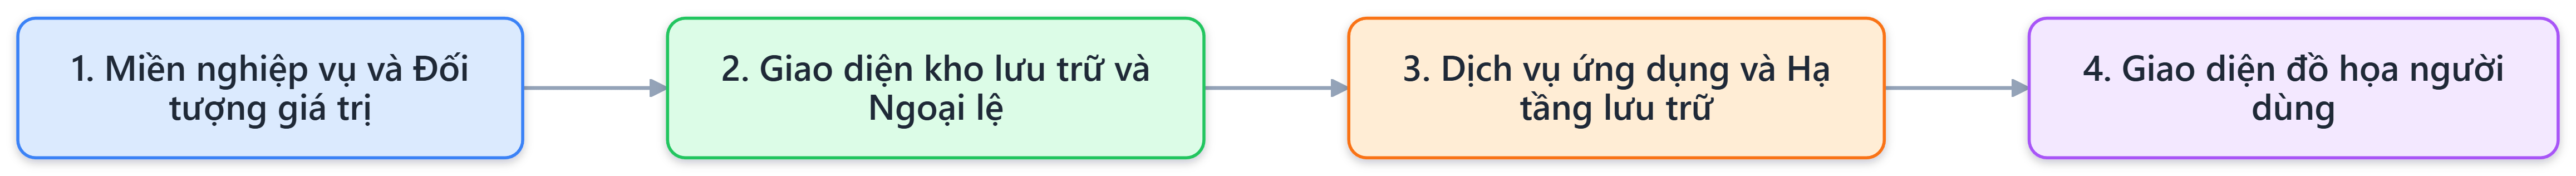
\includegraphics[width=0.85\linewidth,height=\textheight,keepaspectratio,alt={Bối
cảnh chuyển giao từ mô hình thiết kế sang mã nguồn thực
tế}]{./imgs/bao-cao-milestone-4-1.png}
\caption{Bối cảnh chuyển giao từ mô hình thiết kế sang mã nguồn thực tế}
\end{figure}

Trật tự triển khai gồm 4 giai đoạn nối tiếp: 1. Xây dựng nền tảng nghiệp
vụ cốt lõi: Triển khai các đối tượng giá trị bất biến gồm tiền tệ, ngày
giao dịch, tên định danh và cây ngoại lệ nghiệp vụ. Các thực thể miền
gồm ví tiền, danh mục, giao dịch được đóng gói hoàn toàn, không phụ
thuộc vào bất kỳ công nghệ lưu trữ hay giao diện hiển thị nào. 2. Thiết
lập hợp đồng lưu trữ và ngoại lệ: Định nghĩa giao diện kho lưu trữ tổng
quát với kiểu dữ liệu tham số hóa cùng các giao diện kho lưu trữ chuyên
biệt tại tầng miền
(\passthrough{\lstinline!com.pfms.domain.repository!}). 3. Điều phối
nghiệp vụ và cài đặt hạ tầng: Xây dựng các lớp dịch vụ thực thi làm
nhiệm vụ phối hợp các thao tác nguyên tử hai pha và đối soát dữ liệu.
Cài đặt kho lưu trữ tệp JSON với kỹ thuật ghi nguyên tử qua tệp tạm để
chống hỏng dữ liệu khi có sự cố nguồn điện. 4. Hoàn thiện tầng trình
diễn đồ họa: Hiện thực hóa giao diện máy tính để bàn bằng JavaFX 17 theo
kiến trúc phân tách hiển thị và tổ chức mã nguồn theo từng nhóm tính
năng độc lập.

\section{Môi trường thực thi và thư viện công
nghệ}\label{muxf4i-trux1b0ux1eddng-thux1ef1c-thi-vuxe0-thux1b0-viux1ec7n-cuxf4ng-nghux1ec7}

Hệ thống được xây dựng và quản lý thống nhất thông qua công cụ quản lý
dự án Maven với các thông số cấu hình chuẩn mực:

{\def\LTcaptype{none} % do not increment counter
\begin{longtable}[]{@{}
  >{\raggedright\arraybackslash}p{(\linewidth - 4\tabcolsep) * \real{0.3333}}
  >{\raggedright\arraybackslash}p{(\linewidth - 4\tabcolsep) * \real{0.3333}}
  >{\raggedright\arraybackslash}p{(\linewidth - 4\tabcolsep) * \real{0.3333}}@{}}
\toprule\noalign{}
\begin{minipage}[b]{\linewidth}\raggedright
Thành phần công nghệ
\end{minipage} & \begin{minipage}[b]{\linewidth}\raggedright
Phiên bản sử dụng
\end{minipage} & \begin{minipage}[b]{\linewidth}\raggedright
Mục đích và vai trò kỹ thuật
\end{minipage} \\
\midrule\noalign{}
\endhead
\bottomrule\noalign{}
\endlastfoot
\textbf{Ngôn ngữ lập trình} & Java 17 LTS & Khai thác các tính năng hiện
đại như Records, so khớp mẫu, biểu thức chuyển mạch và thư viện thời
gian \passthrough{\lstinline!java.time!}. \\
\textbf{Thư viện giao diện} & OpenJFX 17.0.10 & Cung cấp các thành phần
đồ họa gồm điều khiển giao diện, đồ họa hiển thị và nền tảng sự kiện. \\
\textbf{Công cụ xây dựng dự án} & Apache Maven 3.9+ & Tự động hóa quá
trình biên dịch, chạy toàn bộ bộ kiểm thử và đóng gói tệp thực thi độc
lập kèm thư viện phụ thuộc. \\
\textbf{Khung kiểm thử đơn vị} & JUnit Jupiter 5.10.2 & Thực thi kiểm
thử đơn vị độc lập, kiểm thử tham số hóa và kiểm tra cấu trúc mã
nguồn. \\
\textbf{Thư viện giả lập phụ thuộc} & Mockito 5.11.0 & Giả lập hành vi
của các giao diện kho lưu trữ khi kiểm thử độc lập tầng dịch vụ và tầng
giao diện. \\
\textbf{Xử lý tệp dữ liệu} & Google Gson 2.10.1 & Chuyển đổi hai chiều
giữa thực thể miền và định dạng tệp JSON phẳng theo chuẩn công nghiệp
RFC 8259. \\
\end{longtable}
}

Trình biên dịch Java được thiết lập cờ kiểm tra nghiêm ngặt
\passthrough{\lstinline!-Xlint:all,-serial!} nhằm phát hiện sớm các nguy
cơ tiềm ẩn và loại bỏ hoàn toàn các cảnh báo mã lỗi lỗi thời.

\chapter{Thiết kế Bao gói và Đối tượng Giá trị Bất
biến}\label{thiux1ebft-kux1ebf-bao-guxf3i-vuxe0-ux111ux1ed1i-tux1b0ux1ee3ng-giuxe1-trux1ecb-bux1ea5t-biux1ebfn}

Phần này đặc tả thiết kế bao gói dữ liệu và các đối tượng giá trị bất
biến trong tầng nghiệp vụ của hệ thống PFMS. Trọng tâm cài đặt hướng tới
việc che giấu trạng thái nội tại của các thực thể miền, triệt tiêu sai
số số học tài chính bằng các phép toán bất biến trên kiểu số thực lớn,
và thiết lập hàng rào tiền điều kiện nhằm ngăn chặn dữ liệu sai lệch xâm
nhập vào hệ thống.

\section{Nguyên lý bao gói và che giấu trạng thái nội
tại}\label{nguyuxean-luxfd-bao-guxf3i-vuxe0-che-giux1ea5u-trux1ea1ng-thuxe1i-nux1ed9i-tux1ea1i}

Các thực thể \passthrough{\lstinline!Wallet!},
\passthrough{\lstinline!Category!},
\passthrough{\lstinline!Transaction!} triệt để tuân thủ nguyên lý che
giấu thông tin: - Mọi thuộc tính dữ liệu đều mang phạm vi
\passthrough{\lstinline!private!}. Các trường định danh
\passthrough{\lstinline!id!} và thời điểm tạo lập mang từ khóa
\passthrough{\lstinline!final!} để cố định danh tính thực thể suốt vòng
đời. - Hệ thống loại bỏ hoàn toàn các phương thức gán giá trị tự do
(\passthrough{\lstinline!setter!}). Mọi thay đổi trạng thái được đóng
gói trong các phương thức nghiệp vụ: ví tiền điều chỉnh số dư thông qua
hai phương thức hạch toán \passthrough{\lstinline!credit!} và
\passthrough{\lstinline!debit!} có kiểm tra ràng buộc số dư không âm;
danh mục thực hiện đổi tên và xóa an toàn có kiểm soát.

\section{Cài đặt các đối tượng giá trị bất biến và số học tài chính
chính
xác}\label{cuxe0i-ux111ux1eb7t-cuxe1c-ux111ux1ed1i-tux1b0ux1ee3ng-giuxe1-trux1ecb-bux1ea5t-biux1ebfn-vuxe0-sux1ed1-hux1ecdc-tuxe0i-chuxednh-chuxednh-xuxe1c}

Các đối tượng giá trị được khai báo \passthrough{\lstinline!final!} ở
cấp lớp, mọi trường dữ liệu đều là
\passthrough{\lstinline!private final!}, không cung cấp phương thức thay
đổi trạng thái và mọi phép toán đều trả về thể hiện mới:

\begin{enumerate}
\def\labelenumi{\arabic{enumi}.}
\tightlist
\item
  Lớp tiền tệ \passthrough{\lstinline!Money!}: Đóng gói
  \passthrough{\lstinline!BigDecimal!} với thang đo cố định 2 chữ số
  thập phân (\passthrough{\lstinline!COMPUTATION\_SCALE = 2!}) và quy
  tắc làm tròn nửa chẵn
  (\passthrough{\lstinline!RoundingMode.HALF\_EVEN!}), loại bỏ hoàn toàn
  sai số của kiểu số thực dấu phẩy động \passthrough{\lstinline!float!}
  và \passthrough{\lstinline!double!}. Các phép toán số học như cộng
  (\passthrough{\lstinline!add!}) và trừ
  (\passthrough{\lstinline!subtract!}) luôn trả về một thể hiện
  \passthrough{\lstinline!Money!} mới. Việc tạo mới đối tượng được định
  tuyến qua các phương thức tĩnh như \passthrough{\lstinline!Money.of!}
  và \passthrough{\lstinline!Money.zero!}. Lớp hiện thực hóa
  \passthrough{\lstinline!Comparable<Money>!}, ghi đè đầy đủ
  \passthrough{\lstinline!equals!} và \passthrough{\lstinline!hashCode!}
  theo giá trị số học.
\item
  Lớp ngày giao dịch \passthrough{\lstinline!TransactionDate!}: Đóng gói
  \passthrough{\lstinline!LocalDate!}, xác thực ngày giao dịch không
  được rỗng và không được vượt quá ngày hiện tại của hệ thống. Lớp cung
  cấp phương thức khởi tạo tĩnh và định dạng chuỗi ngày tháng chuẩn phục
  vụ lưu trữ tệp.
\item
  Các lớp chuỗi chuẩn hóa \passthrough{\lstinline!EntityName!} và
  \passthrough{\lstinline!Note!}: \passthrough{\lstinline!EntityName!}
  thực thi quy tắc ràng buộc tên định danh bằng cách cắt tỉa khoảng
  trắng, giới hạn độ dài từ 1 đến 50 ký tự và sinh khóa chuẩn hóa chữ
  thường để kiểm tra trùng lặp không phân biệt hoa thường.
  \passthrough{\lstinline!Note!} chuẩn hóa giá trị rỗng và giới hạn tối
  đa 500 ký tự.
\end{enumerate}

\section{Kiểm soát tiền điều kiện bảo vệ trạng thái hệ
thống}\label{kiux1ec3m-souxe1t-tiux1ec1n-ux111iux1ec1u-kiux1ec7n-bux1ea3o-vux1ec7-trux1ea1ng-thuxe1i-hux1ec7-thux1ed1ng}

Lớp tiện ích \passthrough{\lstinline!Preconditions!} có hàm khởi tạo
\passthrough{\lstinline!private!} nhằm ngăn chặn việc tạo thể hiện, cung
cấp các phương thức tĩnh kiểm tra tham số đầu vào theo nguyên tắc phát
hiện lỗi sớm: - Kiểm tra chuỗi hợp lệ qua
\passthrough{\lstinline!requireNonBlank!}. - Kiểm tra số tiền lớn hơn
không qua \passthrough{\lstinline!requirePositive!} và kiểm tra số dư
không âm qua \passthrough{\lstinline!requireNonNegative!}.

Mọi vi phạm tiền điều kiện đều ném ngay ngoại lệ
\passthrough{\lstinline!IllegalArgumentException!} trước khi tham số
được chuyển vào logic xử lý nội bộ của thực thể hoặc dịch vụ.

\chapter{Kế thừa, Đa hình và Quan hệ Cấu trúc giữa các Thực
thể}\label{kux1ebf-thux1eeba-ux111a-huxecnh-vuxe0-quan-hux1ec7-cux1ea5u-truxfac-giux1eefa-cuxe1c-thux1ef1c-thux1ec3}

Phần này đặc tả việc hiện thực hóa các mối quan hệ cấu trúc hướng đối
tượng cốt lõi trong hệ thống PFMS. Kiến trúc miền nghiệp vụ khai thác kế
thừa để tái sử dụng mã nguồn, áp dụng đa hình động để xử lý biến động
dòng tiền thống nhất, và phân định rạch ròi giữa quan hệ hợp thành sinh
tử và quan hệ kết tập phân cấp.

\section{Cây kế thừa giao dịch tài
chính}\label{cuxe2y-kux1ebf-thux1eeba-giao-dux1ecbch-tuxe0i-chuxednh}

Hệ thống xây dựng mô hình kế thừa phân cấp cho toàn bộ các phát sinh
biến động tiền tệ nhằm tối ưu hóa tính mở rộng và tái sử dụng mã nguồn:

\begin{figure}
\centering
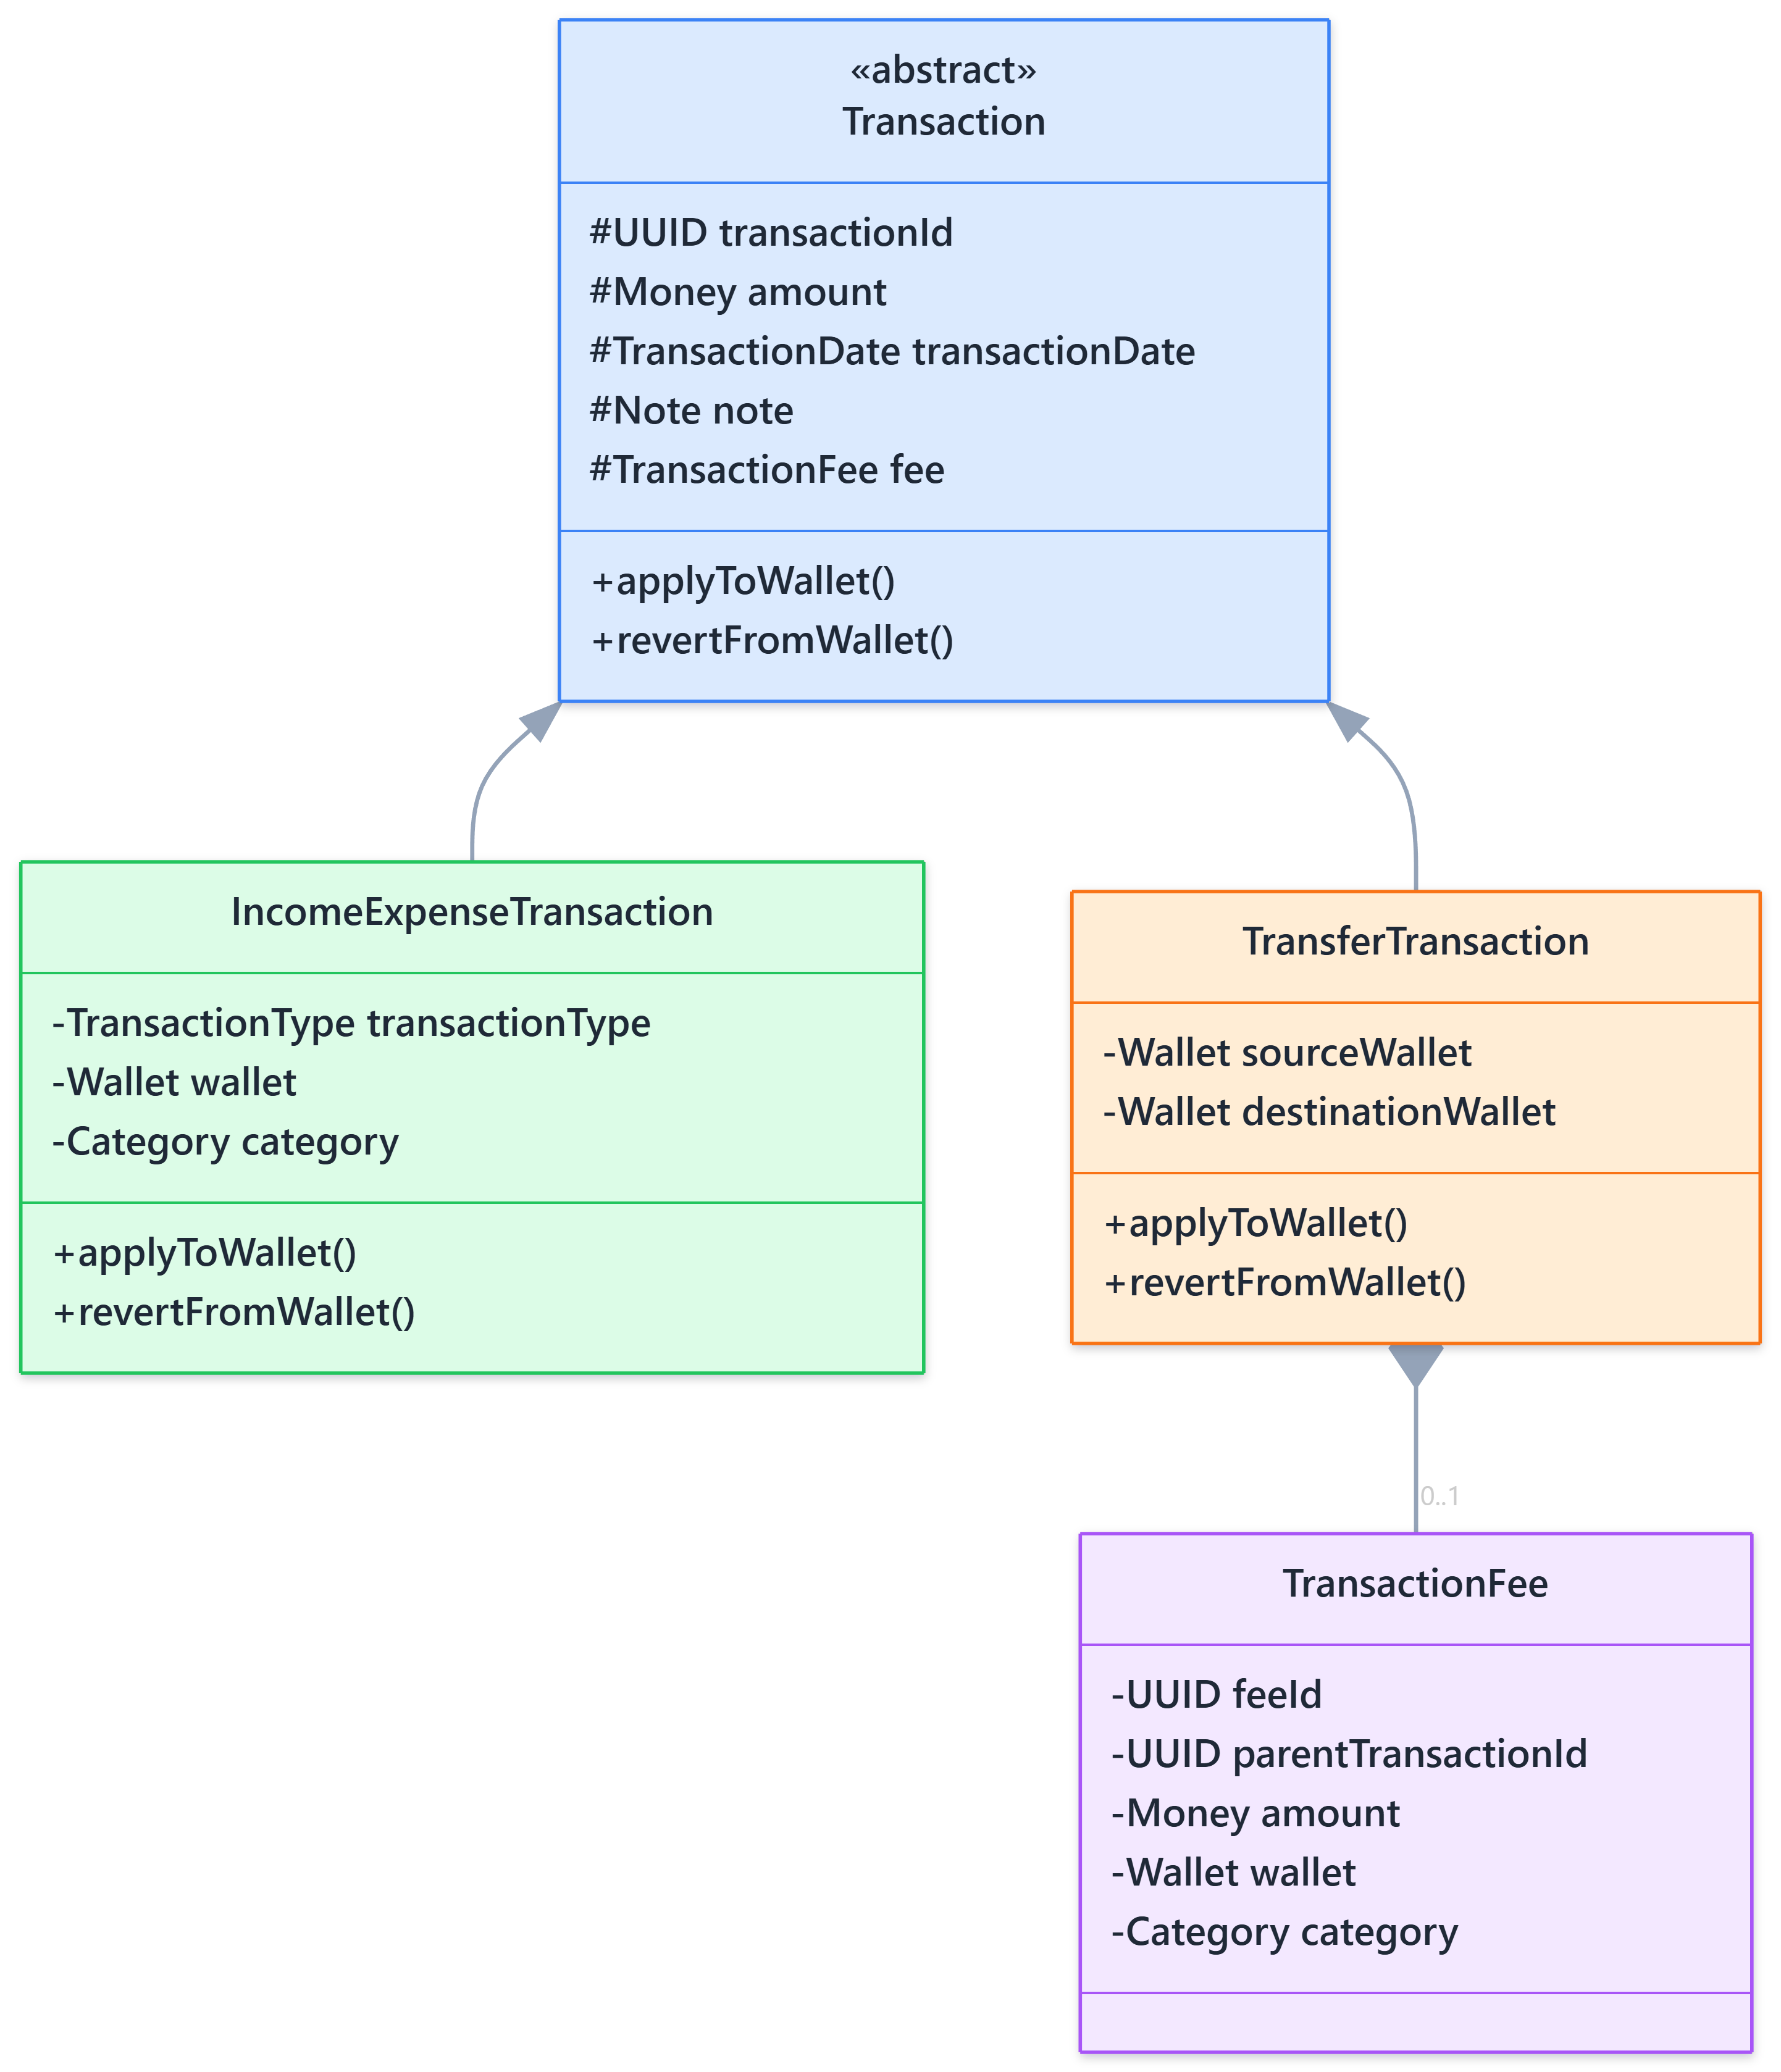
\includegraphics[width=0.85\linewidth,height=\textheight,keepaspectratio,alt={Mô
hình cây kế thừa giao dịch tài chính}]{./imgs/bao-cao-milestone-4-2.png}
\caption{Mô hình cây kế thừa giao dịch tài chính}
\end{figure}

Lớp cha trừu tượng \passthrough{\lstinline!Transaction!} đóng vai trò
khung cơ sở định nghĩa các thuộc tính chung của mọi dòng tiền: mã định
danh, số tiền giao dịch, ngày hạch toán, ghi chú diễn giải, thông tin
phí và thời điểm tạo lập. Lớp cha chứa logic xác thực số tiền dương và
bảo đảm ngày giao dịch không vượt quá thời điểm hiện tại.

Hai lớp con kế thừa cụ thể hóa hai loại biến động tài chính trong thực
tế: - Lớp \passthrough{\lstinline!IncomeExpenseTransaction!}: Bổ sung
thông tin loại thu chi (thu nhập hoặc chi phí), liên kết ví tiền phát
sinh và danh mục phân loại tương ứng. - Lớp
\passthrough{\lstinline!TransferTransaction!}: Bổ sung liên kết giữa ví
nguồn và ví đích, áp dụng kiểm tra bắt buộc ví nguồn và ví đích phải là
hai ví hoàn toàn khác nhau.

\section{Hiện thực hóa tính đa hình trong hạch toán và tính toán dòng
tiền}\label{hiux1ec7n-thux1ef1c-huxf3a-tuxednh-ux111a-huxecnh-trong-hux1ea1ch-touxe1n-vuxe0-tuxednh-touxe1n-duxf2ng-tiux1ec1n}

Tính đa hình động được hiện thực hóa thông qua cặp phương thức trừu
tượng \passthrough{\lstinline!applyToWallet!} và
\passthrough{\lstinline!revertFromWallet!} khai báo tại lớp cha
\passthrough{\lstinline!Transaction!}:

\begin{enumerate}
\def\labelenumi{\arabic{enumi}.}
\tightlist
\item
  Hạch toán ghi nhận dòng tiền qua
  \passthrough{\lstinline!applyToWallet!}:
\end{enumerate}

\begin{itemize}
\tightlist
\item
  Khi thực thi trên \passthrough{\lstinline!IncomeExpenseTransaction!}:
  Nếu là giao dịch thu, hệ thống tự động gọi lệnh cộng tiền
  (\passthrough{\lstinline!credit!}) vào ví. Nếu là giao dịch chi, hệ
  thống tự động gọi lệnh trừ tiền (\passthrough{\lstinline!debit!}) số
  tiền chi tiêu kèm phí phát sinh nếu có.
\item
  Khi thực thi trên \passthrough{\lstinline!TransferTransaction!}: Hệ
  thống đồng thời kiểm tra số dư khả dụng tại ví nguồn, thực hiện trừ
  tổng số tiền chuyển cùng phí khỏi ví nguồn, và cộng đúng số tiền
  chuyển vào ví đích trong cùng một ngữ cảnh giao dịch.
\end{itemize}

\begin{enumerate}
\def\labelenumi{\arabic{enumi}.}
\setcounter{enumi}{1}
\tightlist
\item
  Hoàn tác dòng tiền khi xóa hoặc cập nhật qua
  \passthrough{\lstinline!revertFromWallet!}:
\end{enumerate}

\begin{itemize}
\tightlist
\item
  Khi thực thi trên \passthrough{\lstinline!IncomeExpenseTransaction!}:
  Hệ thống tự động đảo ngược dòng tiền bằng cách trừ tiền đối với giao
  dịch thu nhập cũ hoặc hoàn lại tiền đối với giao dịch chi phí cũ.
\item
  Khi thực thi trên \passthrough{\lstinline!TransferTransaction!}: Hệ
  thống tự động hoàn lại số tiền chuyển và phí về ví nguồn, đồng thời
  khấu trừ số tiền tương ứng khỏi ví đích.
\end{itemize}

Lợi ích kỹ thuật của cơ chế đa hình: Tầng dịch vụ và các thuật toán tổng
hợp báo cáo chỉ cần thao tác trên danh sách các đối tượng kiểu cha
\passthrough{\lstinline!Transaction!}. Hệ thống tự động định tuyến hành
vi hạch toán chính xác tại thời điểm thực thi mà hoàn toàn không cần sử
dụng các khối lệnh kiểm tra kiểu dữ liệu
\passthrough{\lstinline!instanceof!} hay rẽ nhánh điều kiện thủ công.

\section{Quan hệ hợp thành giữa giao dịch chuyển tiền và phí giao
dịch}\label{quan-hux1ec7-hux1ee3p-thuxe0nh-giux1eefa-giao-dux1ecbch-chuyux1ec3n-tiux1ec1n-vuxe0-phuxed-giao-dux1ecbch}

Khoản phí phát sinh khi chuyển tiền nội bộ được mô hình hóa thông qua
lớp \passthrough{\lstinline!TransactionFee!} và gắn kết với
\passthrough{\lstinline!TransferTransaction!} theo quan hệ hợp thành
chặt chẽ: - Ràng buộc vòng đời sinh tử: Một đối tượng
\passthrough{\lstinline!TransactionFee!} không thể tồn tại độc lập mà
bắt buộc phải gắn liền với mã định danh của giao dịch chuyển tiền mẹ. -
Đồng bộ hạch toán và hủy bỏ: Toàn bộ chi phí chuyển tiền được khấu trừ
trực tiếp từ ví nguồn của giao dịch chuyển tiền. Khi một giao dịch
chuyển tiền bị xóa hoặc hoàn tác, bản ghi chi phí đi kèm được tự động xử
lý hoàn tiền về ví nguồn, bảo đảm tính cân bằng số học tuyệt đối.

\section{Quan hệ kết tập trong cây danh mục thu chi ba
cấp}\label{quan-hux1ec7-kux1ebft-tux1eadp-trong-cuxe2y-danh-mux1ee5c-thu-chi-ba-cux1ea5p}

Cấu trúc phân loại tài chính được tổ chức theo mô hình cây ba cấp chuẩn
mực thông qua quan hệ kết tập lỏng giữa các thực thể: - Cấp 1 (Loại biến
động): Phân định giữa hai luồng tiền cơ bản là Thu nhập và Chi phí qua
kiểu liệt kê \passthrough{\lstinline!TransactionType!}. - Cấp 2 (Nhóm
nhu cầu): Lớp \passthrough{\lstinline!NeedGroup!} đại diện cho các nhóm
chi tiêu như nhu cầu thiết yếu, nhu cầu linh hoạt hoặc tích lũy đầu tư.
- Cấp 3 (Danh mục chi tiết): Lớp \passthrough{\lstinline!Category!} đại
diện cho các khoản mục chi tiêu cụ thể như ăn uống, nhà ở, học tập hoặc
phương tiện.

Mối quan hệ giữa danh mục và nhóm nhu cầu là quan hệ kết tập: một danh
mục nắm giữ tham chiếu đến nhóm nhu cầu tương ứng, nhưng nhóm nhu cầu
tồn tại độc lập với vòng đời của từng danh mục con. Khi một danh mục chi
tiết bị xóa mềm, nhóm nhu cầu cha vẫn hoạt động bình thường và không bị
ảnh hưởng.

\chapter{Giao diện Trừu tượng và Kho Lưu trữ Tổng
quát}\label{giao-diux1ec7n-trux1eebu-tux1b0ux1ee3ng-vuxe0-kho-lux1b0u-trux1eef-tux1ed5ng-quuxe1t}

Phần này đặc tả việc thiết kế các giao diện trừu tượng và kho lưu trữ dữ
liệu trong hệ thống PFMS. Kiến trúc tầng dữ liệu áp dụng mẫu kho lưu trữ
kết hợp kỹ thuật kiểu dữ liệu tham số hóa nhằm tách biệt hoàn toàn các
quy tắc nghiệp vụ khỏi chi tiết lưu trữ vật lý, đồng thời thiết lập cơ
chế ghi tệp an toàn chống hỏng dữ liệu trong môi trường máy tính để bàn
cục bộ.

\section{Thiết kế giao diện kho lưu trữ tổng quát với kiểu dữ liệu tham
số
hóa}\label{thiux1ebft-kux1ebf-giao-diux1ec7n-kho-lux1b0u-trux1eef-tux1ed5ng-quuxe1t-vux1edbi-kiux1ec3u-dux1eef-liux1ec7u-tham-sux1ed1-huxf3a}

Hệ thống định nghĩa giao diện cơ sở
\passthrough{\lstinline!GenericRepository<E, ID>!} với hai tham số kiểu
dữ liệu là kiểu thực thể \passthrough{\lstinline!E!} và kiểu khóa nhận
dạng \passthrough{\lstinline!ID!}. Thiết kế này chuẩn hóa toàn bộ các
thao tác dữ liệu cơ bản cho mọi thực thể miền mà không cần viết lại mã
nguồn: - Thao tác lưu trữ: Phương thức \passthrough{\lstinline!save!}
tiếp nhận thực thể và trả về thực thể đã được lưu. Phương thức mặc định
\passthrough{\lstinline!saveAll!} hỗ trợ lưu hàng loạt danh sách thực
thể và trả về danh sách chỉ đọc. - Thao tác truy vấn theo khóa: Phương
thức \passthrough{\lstinline!findById!} nhận mã định danh và trả về đối
tượng \passthrough{\lstinline!Optional<E>!}, bảo đảm an toàn trước lỗi
tham chiếu rỗng. - Thao tác truy vấn toàn phần: Phương thức
\passthrough{\lstinline!findAll!} trả về toàn bộ danh sách thực thể hiện
có. - Thao tác xóa và kiểm tra tồn tại: Phương thức
\passthrough{\lstinline!deleteById!} thực hiện xóa thực thể theo khóa
nhận dạng và trả về kết quả thành công, phương thức
\passthrough{\lstinline!existsById!} kiểm tra sự hiện diện của bản ghi.

Việc sử dụng kiểu dữ liệu tham số hóa giúp mã nguồn đạt tính an toàn
kiểu tại thời điểm biên dịch, loại bỏ hoàn toàn các thao tác ép kiểu thủ
công tiềm ẩn rủi ro lỗi thời gian chạy.

\section{Các giao diện kho lưu trữ nghiệp vụ chuyên
biệt}\label{cuxe1c-giao-diux1ec7n-kho-lux1b0u-trux1eef-nghiux1ec7p-vux1ee5-chuyuxean-biux1ec7t}

Từ giao diện cơ sở, hệ thống mở rộng thành các giao diện kho lưu trữ
chuyên biệt bổ sung các phương thức truy vấn nghiệp vụ đặc thù: - Giao
diện \passthrough{\lstinline!WalletRepository!}: Kế thừa
\passthrough{\lstinline!GenericRepository<Wallet, UUID>!}, bổ sung
phương thức tìm kiếm ví theo tên \passthrough{\lstinline!findByName!}
phục vụ kiểm tra trùng lặp và phương thức
\passthrough{\lstinline!findDefaultWallet!} trích xuất ví mặc định của
hệ thống. - Giao diện \passthrough{\lstinline!TransactionRepository!}:
Kế thừa \passthrough{\lstinline!GenericRepository<Transaction, UUID>!},
bổ sung các phương thức truy vấn lọc theo mã ví, lọc theo danh mục chi
tiêu và lọc giao dịch theo khoảng ngày phát sinh. - Giao diện
\passthrough{\lstinline!CategoryRepository!}: Kế thừa
\passthrough{\lstinline!GenericRepository<Category, UUID>!}, bổ sung
phương thức tra cứu danh mục theo tên và phương thức truy vấn danh sách
danh mục trực thuộc một nhóm nhu cầu cụ thể.

Mọi phương thức trong tầng dịch vụ chỉ giao tiếp thông qua các giao diện
trừu tượng này, bảo đảm sự phụ thuộc lỏng lẻo và độc lập với công nghệ
lưu trữ.

\section{Hiện thực hóa cơ chế lưu trữ tệp an toàn và lưu trữ bộ nhớ kiểm
thử}\label{hiux1ec7n-thux1ef1c-huxf3a-cux1a1-chux1ebf-lux1b0u-trux1eef-tux1ec7p-an-touxe0n-vuxe0-lux1b0u-trux1eef-bux1ed9-nhux1edb-kiux1ec3m-thux1eed}

Hệ thống xây dựng hai cơ chế cài đặt hạ tầng đáp ứng hai mục tiêu vận
hành khác nhau:

\begin{enumerate}
\def\labelenumi{\arabic{enumi}.}
\tightlist
\item
  Cơ chế lưu trữ tệp tin an toàn: Các lớp kho lưu trữ tệp như
  \passthrough{\lstinline!JsonWalletRepository!} và
  \passthrough{\lstinline!JsonTransactionRepository!} đọc và ghi dữ liệu
  ra các tệp tin có cấu trúc trên ổ đĩa. Quá trình ghi tệp được bảo vệ
  qua cơ chế ghi nguyên tử:
\end{enumerate}

\begin{itemize}
\tightlist
\item
  Dữ liệu trước tiên được tuần tự hóa và ghi vào một tệp tạm thời có
  phần mở rộng \passthrough{\lstinline!.tmp!} trong cùng thư mục đích.
\item
  Sau khi quá trình ghi tệp tạm hoàn tất không có lỗi, hệ thống mới thực
  hiện thao tác tráo đổi nguyên tử để tệp tạm thay thế tệp chính.
\item
  Nếu xảy ra sự cố đột ngột về mất điện hoặc gián đoạn tiến trình trong
  khi đang ghi, tệp chính trước đó vẫn được bảo toàn nguyên vẹn, triệt
  tiêu hoàn toàn rủi ro tệp dữ liệu bị cắt cụt hoặc hỏng cấu trúc.
\end{itemize}

\begin{enumerate}
\def\labelenumi{\arabic{enumi}.}
\setcounter{enumi}{1}
\tightlist
\item
  Cơ chế lưu trữ bộ nhớ phục vụ kiểm thử: Các lớp kho lưu trữ bộ nhớ
  quản lý dữ liệu trực tiếp trong các cấu trúc bảng băm an toàn luồng,
  cho phép thực thi toàn bộ các ca kiểm thử tự động với tốc độ cực nhanh
  mà không phụ thuộc vào tốc độ vào ra của ổ đĩa vật lý.
\end{enumerate}

\chapter{Cấu trúc Dữ liệu Tập hợp và Bảo vệ Dữ
liệu}\label{cux1ea5u-truxfac-dux1eef-liux1ec7u-tux1eadp-hux1ee3p-vuxe0-bux1ea3o-vux1ec7-dux1eef-liux1ec7u}

Phần này đặc tả việc ứng dụng khung tập hợp dữ liệu Java trong toàn bộ
hệ thống PFMS. Trọng tâm cài đặt tập trung vào việc lựa chọn cấu trúc dữ
liệu tối ưu cho từng tác vụ lưu trữ và tra cứu, áp dụng kỹ thuật sao
chép phòng thủ và danh sách bất biến nhằm bảo vệ tuyệt đối dữ liệu nội
tại trước các can thiệp ngoài ý muốn.

\section{Ứng dụng khung tập hợp dữ liệu trong quản lý và truy xuất thực
thể}\label{ux1ee9ng-dux1ee5ng-khung-tux1eadp-hux1ee3p-dux1eef-liux1ec7u-trong-quux1ea3n-luxfd-vuxe0-truy-xuux1ea5t-thux1ef1c-thux1ec3}

Hệ thống lựa chọn chính xác các giao diện và lớp triển khai trong khung
tập hợp dữ liệu phù hợp với đặc thù nghiệp vụ tài chính: - Giao diện
danh sách \passthrough{\lstinline!List!} qua lớp
\passthrough{\lstinline!ArrayList!}: Được sử dụng làm cấu trúc lưu trữ
chủ đạo cho lịch sử giao dịch và kết quả truy vấn. Danh sách bảo toàn
chính xác thứ tự phát sinh dòng tiền theo thời gian, cho phép truy xuất
phần tử theo chỉ số và hỗ trợ hiệu quả cho thuật toán phân trang dữ liệu
trên giao diện. - Giao diện ánh xạ \passthrough{\lstinline!Map!} qua lớp
\passthrough{\lstinline!ConcurrentHashMap!}: Được ứng dụng trong các kho
lưu trữ bộ nhớ và các bộ đối soát dữ liệu. Cấu trúc này liên kết khóa
nhận dạng duy nhất với thể hiện thực thể, cho phép tìm kiếm bản ghi với
độ phức tạp thời gian hằng số và bảo đảm an toàn luồng khi xử lý đa tác
vụ. - Giao diện tập hợp duy nhất \passthrough{\lstinline!Set!} qua lớp
\passthrough{\lstinline!HashSet!}: Được sử dụng để quản lý tập hợp các
khóa tên định danh đã được chuẩn hóa và loại bỏ các phần tử trùng lặp
khi tổng hợp danh mục báo cáo.

\section{Kỹ thuật bảo vệ dữ liệu với danh sách bất biến và sao chép
phòng
thủ}\label{kux1ef9-thuux1eadt-bux1ea3o-vux1ec7-dux1eef-liux1ec7u-vux1edbi-danh-suxe1ch-bux1ea5t-biux1ebfn-vuxe0-sao-chuxe9p-phuxf2ng-thux1ee7}

Để duy trì tính toàn vẹn của mô hình hướng đối tượng, hệ thống áp dụng
nghiêm ngặt hai kỹ thuật bảo vệ tập hợp dữ liệu: 1. Kỹ thuật sao chép
phòng thủ: Khi một thực thể hoặc phương thức dịch vụ tiếp nhận một tập
hợp từ bên ngoài, hệ thống luôn khởi tạo một bản sao mới độc lập trước
khi gán cho thuộc tính nội bộ. Thao tác này ngăn chặn hoàn toàn việc bên
ngoài tiếp tục sửa đổi danh sách gốc làm thay đổi trạng thái bên trong
thực thể. 2. Danh sách bất biến qua
\passthrough{\lstinline!Collections.unmodifiableList!}: Toàn bộ các
phương thức truy vấn trả về danh sách thực thể tại kho lưu trữ hoặc tầng
dịch vụ đều bọc tập hợp kết quả qua phương thức
\passthrough{\lstinline!Collections.unmodifiableList!}. Bản bọc này tạo
ra một khung nhìn chỉ đọc: tầng giao diện hoặc các thành phần gọi bên
ngoài chỉ có thể duyệt và đọc dữ liệu, mọi nỗ lực can thiệp thêm, sửa
hoặc xóa phần tử đều bị máy ảo Java ném ngoại lệ
\passthrough{\lstinline!UnsupportedOperationException!} ngay lập tức.

\chapter{Cây Phân cấp Ngoại lệ và Cơ chế Kiểm soát
Lỗi}\label{cuxe2y-phuxe2n-cux1ea5p-ngoux1ea1i-lux1ec7-vuxe0-cux1a1-chux1ebf-kiux1ec3m-souxe1t-lux1ed7i}

Phần này đặc tả kiến trúc quản lý ngoại lệ và cơ chế kiểm soát lỗi trong
hệ thống PFMS. Hệ thống xây dựng cây phân cấp ngoại lệ có cấu trúc chặt
chẽ kế thừa từ ngoại lệ thời gian chạy, phân định ranh giới rõ ràng giữa
lỗi nghiệp vụ người dùng và sự cố kỹ thuật hạ tầng, kết hợp từ điển mã
lỗi chuẩn hóa để cung cấp thông điệp cảnh báo thân thiện trên giao diện.

\section{Chiến lược quản lý ngoại lệ toàn hệ
thống}\label{chiux1ebfn-lux1b0ux1ee3c-quux1ea3n-luxfd-ngoux1ea1i-lux1ec7-touxe0n-hux1ec7-thux1ed1ng}

Hệ thống áp dụng chiến lược quản lý ngoại lệ tập trung dựa trên nền tảng
ngoại lệ không bắt buộc: 1. Toàn bộ các ngoại lệ tự định nghĩa trong hệ
thống đều kế thừa từ lớp trừu tượng
\passthrough{\lstinline!PfmsException!} (trực thuộc
\passthrough{\lstinline!RuntimeException!}). Lựa chọn này giúp giữ chữ
ký các phương thức ở tầng miền và tầng dịch vụ luôn sạch sẽ, tránh làm ô
nhiễm mã nguồn bằng các khai báo \passthrough{\lstinline!throws!} không
cần thiết. 2. Hệ thống phân định rạch ròi thành hai nhánh ngoại lệ
chính: - Nhánh ngoại lệ nghiệp vụ
(\passthrough{\lstinline!BusinessException!}): Đại diện cho các vi phạm
quy tắc tài chính hoặc dữ liệu đầu vào của người dùng. Các ngoại lệ này
được bắt tại tầng điều khiển giao diện để hiển thị thông báo hướng dẫn
người dùng điều chỉnh thao tác. - Nhánh ngoại lệ kỹ thuật
(\passthrough{\lstinline!TechnicalException!} và
\passthrough{\lstinline!StorageException!}): Đại diện cho các sự cố hạ
tầng như lỗi vào ra tệp tin, lỗi quyền truy cập thư mục hoặc sai định
dạng tệp lưu trữ trên ổ đĩa.

Mọi thể hiện \passthrough{\lstinline!PfmsException!} đều tự động ghi
nhận mã lỗi chuẩn hóa \passthrough{\lstinline!ErrorCode!} và mốc thời
gian phát sinh sự cố phục vụ việc theo dõi vết lỗi.

\section{Cây phân cấp ngoại lệ nghiệp
vụ}\label{cuxe2y-phuxe2n-cux1ea5p-ngoux1ea1i-lux1ec7-nghiux1ec7p-vux1ee5}

Mô hình phân cấp ngoại lệ được tổ chức theo cấu trúc kế thừa phân tầng:

\begin{figure}
\centering
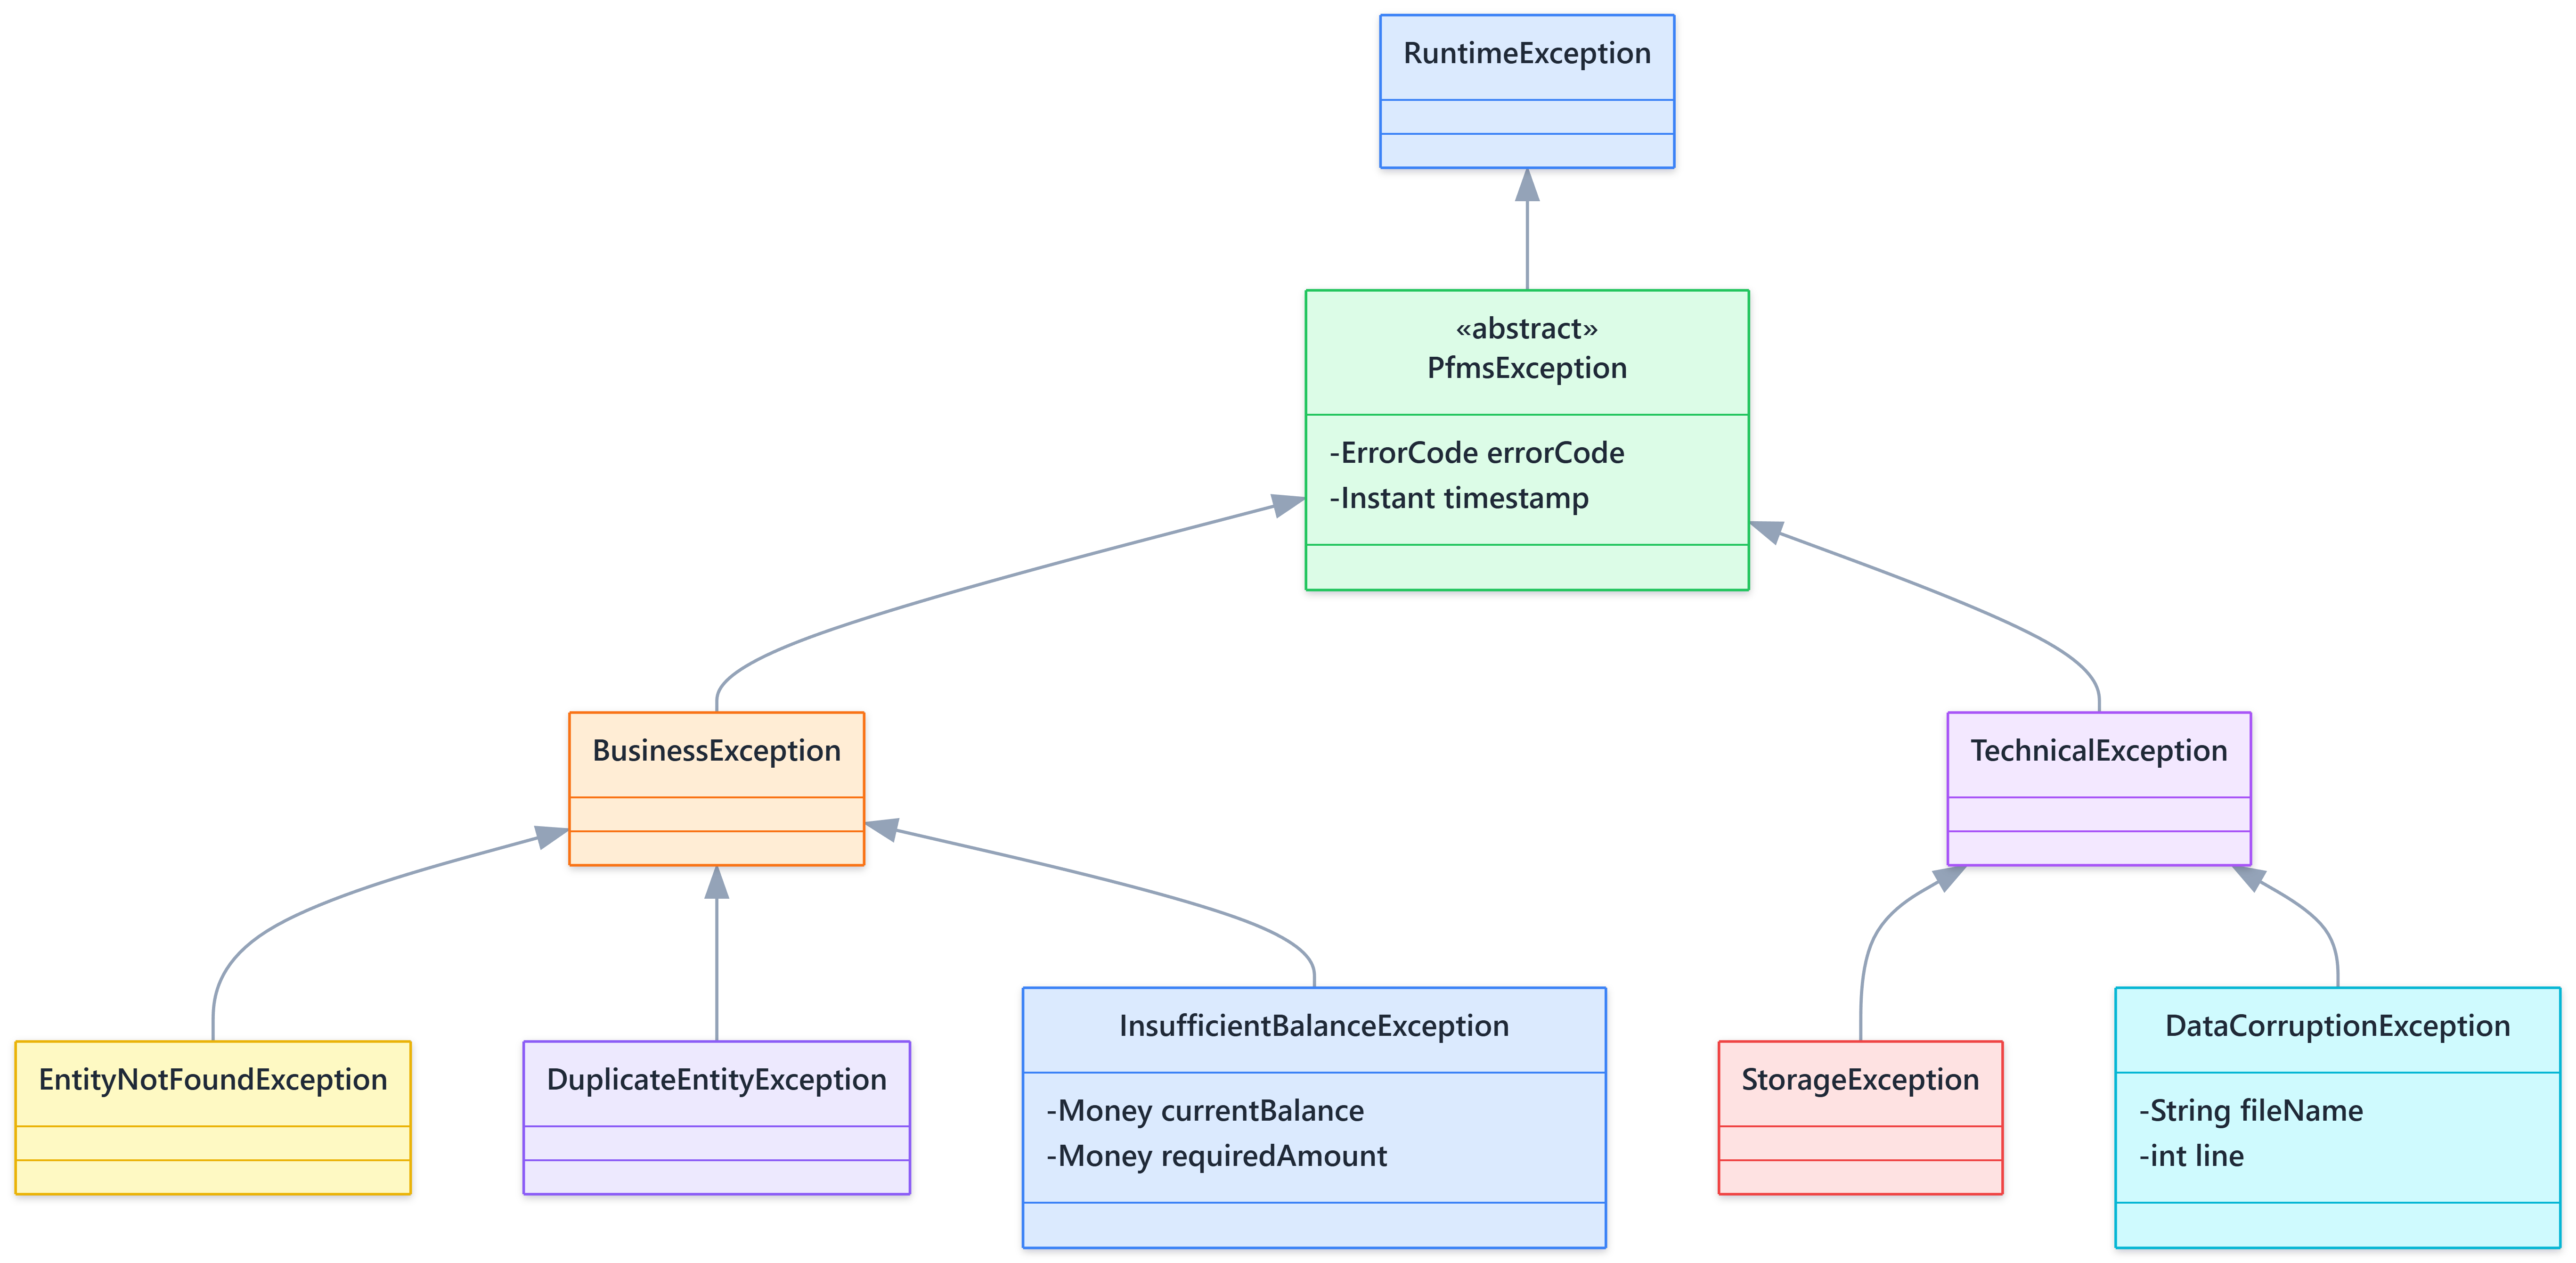
\includegraphics[width=0.85\linewidth,height=\textheight,keepaspectratio,alt={Mô
hình phân cấp cây ngoại lệ nghiệp vụ hệ thống
PFMS}]{./imgs/bao-cao-milestone-4-3.png}
\caption{Mô hình phân cấp cây ngoại lệ nghiệp vụ hệ thống PFMS}
\end{figure}

Các lớp ngoại lệ nghiệp vụ con giải quyết các tình huống lỗi chuyên
biệt: - Ngoại lệ \passthrough{\lstinline!InsufficientBalanceException!}:
Kích hoạt khi ví nguồn không có đủ số dư khả dụng để chi trả khoản
chuyển tiền và phí. Lớp mang theo thông tin số dư hiện tại và số tiền
yêu cầu nhằm hỗ trợ tầng giao diện giải trình nguyên nhân thiếu hụt. -
Ngoại lệ \passthrough{\lstinline!DuplicateEntityException!}: Kích hoạt
khi người dùng cố gắng tạo ví tiền hoặc danh mục có tên đã tồn tại trong
cùng phạm vi quản lý. - Ngoại lệ
\passthrough{\lstinline!EntityNotFoundException!}: Kích hoạt khi tra cứu
thực thể theo mã định danh nhưng không tìm thấy bản ghi tương ứng trong
kho lưu trữ. - Ngoại lệ
\passthrough{\lstinline!DataCorruptionException!}: Kích hoạt trong quá
trình kiểm tra đối soát nếu phát hiện số dư thực tế bị sai lệch so với
tổng các dòng tiền lịch sử hoặc tệp sao lưu có cấu trúc dữ liệu bị cắt
cụt.

\section{Quy chuẩn mã lỗi và chuyển đổi thông điệp cảnh
báo}\label{quy-chuux1ea9n-muxe3-lux1ed7i-vuxe0-chuyux1ec3n-ux111ux1ed5i-thuxf4ng-ux111iux1ec7p-cux1ea3nh-buxe1o}

Hệ thống chuẩn hóa danh mục lỗi thông qua kiểu liệt kê
\passthrough{\lstinline!ErrorCode!}. Mỗi mã lỗi được phân nhóm theo phân
hệ chức năng bằng tiền tố ngắn gọn và gắn liền với một thông điệp tiếng
Việt mặc định rõ ràng: - Nhóm tiền tệ và số học: Định danh các lỗi định
dạng số tiền hoặc chia không xác định quy tắc làm tròn. - Nhóm tên định
danh: Định danh lỗi tên vi phạm giới hạn từ 1 đến 50 ký tự hoặc trùng
lặp tên trong hệ thống. - Nhóm ví tiền và chuyển tiền: Định danh lỗi số
dư không đủ, lỗi chọn trùng ví nguồn và ví đích, hoặc số tiền chuyển
không dương. - Nhóm danh mục và dữ liệu: Định danh các vi phạm ràng buộc
danh mục và lỗi hỏng cấu trúc tệp dữ liệu sao lưu.

Tầng giao diện người dùng JavaFX bắt các ngoại lệ này tại bộ điều khiển,
tự động trích xuất thông điệp mặc định từ mã lỗi và hiển thị qua các hộp
thoại cảnh báo thân thiện, che giấu hoàn toàn các chi tiết kỹ thuật phức
tạp đối với người dùng cuối.

\chapter{Tầng Dịch vụ Ứng dụng và Giao diện Người
dùng}\label{tux1ea7ng-dux1ecbch-vux1ee5-ux1ee9ng-dux1ee5ng-vuxe0-giao-diux1ec7n-ngux1b0ux1eddi-duxf9ng}

Phần này đặc tả việc hiện thực hóa tầng dịch vụ ứng dụng và tầng trình
diễn đồ họa người dùng trong hệ thống PFMS. Tầng dịch vụ đóng vai trò
điều phối các kịch bản sử dụng và bảo toàn tính toàn vẹn tài chính, kết
nối với giao diện đồ họa JavaFX 17 thông qua kiến trúc phân tách hiển
thị và các đối tượng truyền dữ liệu bất biến nhằm ngăn chặn hoàn toàn
việc rò rỉ chi tiết miền ra bên ngoài.

\section{Điều phối nghiệp vụ và bảo toàn giao dịch hai
pha}\label{ux111iux1ec1u-phux1ed1i-nghiux1ec7p-vux1ee5-vuxe0-bux1ea3o-touxe0n-giao-dux1ecbch-hai-pha}

Tầng dịch vụ ứng dụng được phân rã thành 6 giao diện chuyên biệt bảo đảm
tính gắn kết cao: \passthrough{\lstinline!WalletService!},
\passthrough{\lstinline!TransactionService!},
\passthrough{\lstinline!TransferService!},
\passthrough{\lstinline!CategoryService!},
\passthrough{\lstinline!ReportService!} và
\passthrough{\lstinline!DataManagementService!}.

Các cơ chế điều phối nghiệp vụ trọng tâm gồm: 1. Giao dịch chuyển tiền
hai pha nguyên tử: Lớp \passthrough{\lstinline!TransferServiceImpl!}
điều phối quy trình chuyển tiền giữa hai ví độc lập. Thao tác bao gồm
việc thẩm định số dư khả dụng tại ví nguồn, thực hiện trừ số tiền chuyển
cùng phí khỏi ví nguồn và cộng tiền vào ví đích trong cùng một ngữ cảnh.
Nếu phát sinh bất kỳ lỗi lưu trữ nào ở giữa quy trình, cơ chế hỗ trợ
hoàn tác sẽ khôi phục trạng thái số dư ban đầu của cả hai ví, ngăn chặn
hoàn toàn hiện tượng thất thoát dòng tiền một đầu. 2. Kiểm tra đối soát
tính toàn vẹn dữ liệu: Lớp
\passthrough{\lstinline!SystemDataReconciler!} thực hiện quét toàn bộ dữ
liệu lịch sử để kiểm tra tính toàn vẹn số học. Số dư của mỗi ví được
tính toán độc lập từ tổng các giao dịch thu, chi, chuyển tiền và điều
chỉnh số dư trong quá khứ để đối soát với số dư hiện tại, phát hiện sớm
các nguy cơ sai lệch dữ liệu.

\section{Giao diện đồ họa người dùng theo kiến trúc phân tách hiển
thị}\label{giao-diux1ec7n-ux111ux1ed3-hux1ecda-ngux1b0ux1eddi-duxf9ng-theo-kiux1ebfn-truxfac-phuxe2n-tuxe1ch-hiux1ec3n-thux1ecb}

Tầng giao diện đồ họa được xây dựng trên nền tảng JavaFX 17 và tổ chức
mã nguồn theo từng nhóm tính năng độc lập. Hệ thống áp dụng triệt để mô
hình kiến trúc phân tách hiển thị giữa Khung nhìn và Bộ điều phối: - Hợp
đồng hiển thị: Các giao diện như \passthrough{\lstinline!WalletView!} và
\passthrough{\lstinline!TransactionView!} là các hợp đồng thuần Java,
hoàn toàn không chứa thư viện đồ họa JavaFX. Hợp đồng này chỉ định nghĩa
các phương thức cập nhật dữ liệu bảng và hiển thị thông báo. - Bộ điều
phối hiển thị: Các lớp như \passthrough{\lstinline!WalletPresenter!} và
\passthrough{\lstinline!TransactionPresenter!} tiếp nhận dữ liệu từ dịch
vụ, chuyển đổi sang dữ liệu hiển thị và ra lệnh cho khung nhìn cập nhật.
Do không phụ thuộc vào thành phần đồ họa, toàn bộ logic hiển thị của
Presenter được kiểm thử tự động độc lập 100\% trong môi trường không có
màn hình. - Khung nhìn đồ họa: Các lớp như
\passthrough{\lstinline!WalletPane!} và
\passthrough{\lstinline!TransactionPane!} hiện thực hóa hợp đồng hiển
thị bằng các điều khiển giao diện JavaFX hiện đại, chỉ đảm nhiệm việc vẽ
bảng biểu và bắt sự kiện người dùng. - Bộ điều khiển giao diện: Các lớp
như \passthrough{\lstinline!WalletGUIController!} tiếp nhận tương tác
nút bấm, thực hiện kiểm thực biểu mẫu sơ bộ và ủy quyền xử lý cho tầng
dịch vụ tương ứng.

\section{Đối tượng truyền dữ liệu và ranh giới phân
tầng}\label{ux111ux1ed1i-tux1b0ux1ee3ng-truyux1ec1n-dux1eef-liux1ec7u-vuxe0-ranh-giux1edbi-phuxe2n-tux1ea7ng}

Nhằm bảo đảm tính độc lập giữa tầng giao diện và tầng nghiệp vụ, hệ
thống thiết lập ranh giới giao tiếp hoàn toàn thông qua các đối tượng
truyền dữ liệu: - Đối tượng truyền dữ liệu yêu cầu
(\passthrough{\lstinline!RequestDTO!}): Đóng gói toàn bộ tham số người
dùng nhập từ biểu mẫu giao diện trước khi gửi xuống tầng dịch vụ. - Đối
tượng truyền dữ liệu phản hồi (\passthrough{\lstinline!ResponseDTO!}):
Đóng gói kết quả xử lý từ dịch vụ trả về cho bộ điều phối hiển thị.

Cơ chế này ngăn chặn tuyệt đối việc để lộ các thực thể miền ra tầng giao
diện, bảo đảm các thay đổi về bố cục màn hình hay thư viện đồ họa hoàn
toàn không ảnh hưởng đến các quy tắc tài chính cốt lõi bên trong.

\chapter{Kiểm thử Đơn vị Tự động và Đối soát Nghiệm
thu}\label{kiux1ec3m-thux1eed-ux111ux1a1n-vux1ecb-tux1ef1-ux111ux1ed9ng-vuxe0-ux111ux1ed1i-souxe1t-nghiux1ec7m-thu}

Phần này trình bày chiến lược kiểm thử đơn vị tự động và kết quả đối
soát nghiệm thu mã nguồn của hệ thống PFMS. Toàn bộ các quy tắc tài
chính, ràng buộc dữ liệu biên và luồng điều phối ca sử dụng đều được
kiểm chứng độc lập bằng bộ kiểm thử tự động, bảo đảm tính đúng đắn và độ
tin cậy của hệ thống.

\section{Chiến lược kiểm thử đơn vị và ma trận giá trị biên tài
chính}\label{chiux1ebfn-lux1b0ux1ee3c-kiux1ec3m-thux1eed-ux111ux1a1n-vux1ecb-vuxe0-ma-trux1eadn-giuxe1-trux1ecb-biuxean-tuxe0i-chuxednh}

Hệ thống áp dụng phương pháp phát triển hướng kiểm thử theo nguyên tắc
từ trong ra ngoài: 1. Kiểm thử cô lập với bộ nhớ tạm: Toàn bộ các ca
kiểm thử tầng miền và tầng dịch vụ sử dụng kho lưu trữ bộ nhớ và đối
tượng giả lập Mockito, cách ly hoàn toàn với ổ đĩa vật lý để đạt tốc độ
thực thi tối đa. 2. Ma trận kiểm định 5 nhóm giá trị biên tài chính: -
Nhóm biên số tiền: Kiểm tra từ chối số tiền bằng 0 và số tiền âm; kiểm
tra tính toán số tiền cực đại lên đến hàng trăm tỷ đồng bảo đảm không bị
tràn số học trên \passthrough{\lstinline!BigDecimal!}. - Nhóm biên chuỗi
định danh: Kiểm tra tên ví và danh mục tại đúng các mốc giới hạn 1 ký tự
và 50 ký tự; kiểm tra việc tự động cắt tỉa khoảng trắng ở hai đầu chuỗi.
- Nhóm biên bảo toàn số dư: Kiểm tra số dư ví giảm về đúng 0; kiểm tra
việc ném ngoại lệ từ chối chuyển tiền khi số dư ví nguồn nhỏ hơn tổng
tiền chuyển và phí dù chỉ 1 đồng. - Nhóm biên ngày tháng: Kiểm tra tính
hợp lệ của ngày trong quá khứ và ngày hiện tại; kiểm tra việc từ chối
các giao dịch có ngày phát sinh trong tương lai. - Nhóm biên trạng thái
thực thể: Kiểm tra việc từ chối ghi nhận giao dịch vào ví đã đóng hoặc
ví đã xóa; kiểm tra ràng buộc không cho phép xóa danh mục khi đang có
giao dịch phát sinh liên kết.

\section{Bằng chứng thực thi bộ kiểm thử tự
động}\label{bux1eb1ng-chux1ee9ng-thux1ef1c-thi-bux1ed9-kiux1ec3m-thux1eed-tux1ef1-ux111ux1ed9ng}

Quá trình xây dựng và kiểm thử hệ thống được tự động hóa hoàn toàn thông
qua công cụ Maven Surefire. Toàn bộ các ca kiểm thử tự động của dự án
đều vượt qua với trạng thái thành công tuyệt đối, không phát sinh bất kỳ
lỗi biên dịch, lỗi ngoại lệ hay trường hợp thất bại nào.

Bảng phân bổ trọng tâm kiểm thử theo từng phân hệ kiến trúc:

{\def\LTcaptype{none} % do not increment counter
\begin{longtable}[]{@{}
  >{\raggedright\arraybackslash}p{(\linewidth - 2\tabcolsep) * \real{0.5000}}
  >{\raggedright\arraybackslash}p{(\linewidth - 2\tabcolsep) * \real{0.5000}}@{}}
\toprule\noalign{}
\begin{minipage}[b]{\linewidth}\raggedright
Phân hệ mã nguồn
\end{minipage} & \begin{minipage}[b]{\linewidth}\raggedright
Trọng tâm kiểm thử
\end{minipage} \\
\midrule\noalign{}
\endhead
\bottomrule\noalign{}
\endlastfoot
\textbf{Thực thể và Đối tượng giá trị}
(\passthrough{\lstinline!domain.model!}) & Tính toán số học tiền tệ của
\passthrough{\lstinline!Money!}, tính bất biến, các quy tắc số dư và
trạng thái của \passthrough{\lstinline!Wallet!},
\passthrough{\lstinline!Category!},
\passthrough{\lstinline!Transaction!}. \\
\textbf{Ngoại lệ và Tiện ích}
(\passthrough{\lstinline!domain.exception!},
\passthrough{\lstinline!common.util!}) & Ràng buộc kiểm tra tiền điều
kiện của \passthrough{\lstinline!Preconditions!}, ánh xạ thông điệp của
từ điển mã lỗi \passthrough{\lstinline!ErrorCode!}. \\
\textbf{Tầng Dịch vụ ứng dụng} (\passthrough{\lstinline!service!}) &
Luồng điều phối ca sử dụng, chuyển tiền hai pha nguyên tử, đối soát dữ
liệu toàn vẹn, thuật toán tổng hợp dòng tiền. \\
\textbf{Tầng Hạ tầng lưu trữ} (\passthrough{\lstinline!infrastructure!})
& Cơ chế đọc ghi tệp JSON, an toàn tệp qua kỹ thuật ghi nguyên tử với
tệp tạm, phục hồi và kiểm định bản sao lưu. \\
\textbf{Tầng Trình diễn đồ họa} (\passthrough{\lstinline!presentation!})
& Logic hiển thị của bộ điều phối Presenter độc lập với màn hình, kiểm
thực dữ liệu biểu mẫu, đóng gói và chuyển đổi DTO. \\
\end{longtable}
}

\section{Ma trận đối soát ca sử dụng sang mã nguồn dịch
vụ}\label{ma-trux1eadn-ux111ux1ed1i-souxe1t-ca-sux1eed-dux1ee5ng-sang-muxe3-nguux1ed3n-dux1ecbch-vux1ee5}

Toàn bộ 20 ca sử dụng chuẩn hóa từ tài liệu yêu cầu được nghiệm thu khép
kín qua các lớp dịch vụ thực thi tương ứng:

{\def\LTcaptype{none} % do not increment counter
\begin{longtable}[]{@{}
  >{\raggedright\arraybackslash}p{(\linewidth - 4\tabcolsep) * \real{0.3333}}
  >{\raggedright\arraybackslash}p{(\linewidth - 4\tabcolsep) * \real{0.3333}}
  >{\raggedright\arraybackslash}p{(\linewidth - 4\tabcolsep) * \real{0.3333}}@{}}
\toprule\noalign{}
\begin{minipage}[b]{\linewidth}\raggedright
Phân hệ nghiệp vụ
\end{minipage} & \begin{minipage}[b]{\linewidth}\raggedright
Phạm vi ca sử dụng chuẩn hóa
\end{minipage} & \begin{minipage}[b]{\linewidth}\raggedright
Lớp dịch vụ chịu trách nhiệm
\end{minipage} \\
\midrule\noalign{}
\endhead
\bottomrule\noalign{}
\endlastfoot
\textbf{Quản lý ví tiền} & UC-WAL-01 đến UC-WAL-04 (Tạo ví, xem tổng hợp
số dư, cập nhật thông tin, điều chỉnh số dư) &
\passthrough{\lstinline!WalletServiceImpl!} \\
\textbf{Ghi nhận thu chi} & UC-TXN-01 đến UC-TXN-04 (Ghi nhận thu chi,
tra cứu lọc lịch sử, chỉnh sửa, xóa giao dịch) &
\passthrough{\lstinline!TransactionServiceImpl!} \\
\textbf{Chuyển tiền nội bộ} & UC-TRF-01 đến UC-TRF-03 (Chuyển tiền hai
pha, tra cứu lịch sử chuyển tiền, xóa hoàn tác) &
\passthrough{\lstinline!TransferServiceImpl!} \\
\textbf{Danh mục phân loại} & UC-CAT-01 đến UC-CAT-04 (Thêm mới danh
mục, đổi tên, khôi phục, xóa an toàn) &
\passthrough{\lstinline!CategoryServiceImpl!} \\
\textbf{Báo cáo và thống kê} & UC-REP-01 và UC-REP-02 (Thống kê dòng
tiền 12 tháng, phân tích cơ cấu thu chi) &
\passthrough{\lstinline!ReportServiceImpl!} \\
\textbf{Quản trị dữ liệu} & UC-DAT-01 đến UC-DAT-03 (Xuất dữ liệu an
toàn, phục hồi từ bản sao lưu, đối soát dữ liệu) &
\passthrough{\lstinline!DataManagementServiceImpl!} \\
\end{longtable}
}

Kết quả đối soát xác nhận độ bao phủ đạt tính khép kín 100\%: mọi ca sử
dụng đều có lớp dịch vụ thực thi cụ thể đảm nhiệm, không có tính năng
nào bị bỏ sót và không tồn tại mã nguồn mồ côi.

\chapter{Đánh giá Mức độ Hoàn thiện Hệ
thống}\label{ux111uxe1nh-giuxe1-mux1ee9c-ux111ux1ed9-houxe0n-thiux1ec7n-hux1ec7-thux1ed1ng}

Quá trình cài đặt mã nguồn cốt lõi của hệ thống Quản lý Tài chính Cá
nhân PFMS đã hoàn thành toàn diện các yêu cầu kỹ thuật đề ra. Toàn bộ
các nguyên lý thiết kế hướng đối tượng, kiến trúc phân tầng và giải pháp
bảo vệ dữ liệu tài chính đã được hiện thực hóa đầy đủ, đồng bộ và kiểm
chứng nghiêm ngặt qua hệ thống kiểm thử tự động.

{\def\LTcaptype{none} % do not increment counter
\begin{longtable}[]{@{}
  >{\raggedright\arraybackslash}p{(\linewidth - 2\tabcolsep) * \real{0.5000}}
  >{\raggedright\arraybackslash}p{(\linewidth - 2\tabcolsep) * \real{0.5000}}@{}}
\toprule\noalign{}
\begin{minipage}[b]{\linewidth}\raggedright
Trụ cột kỹ thuật
\end{minipage} & \begin{minipage}[b]{\linewidth}\raggedright
Mức độ đáp ứng trong mã nguồn
\end{minipage} \\
\midrule\noalign{}
\endhead
\bottomrule\noalign{}
\endlastfoot
\textbf{Bao gói và Đối tượng giá trị} & Đạt mức độ hoàn thiện tuyệt đối.
100\% trường dữ liệu được bao gói riêng tư
(\passthrough{\lstinline!private final!}). Các đối tượng giá trị bất
biến (\passthrough{\lstinline!Money!},
\passthrough{\lstinline!TransactionDate!},
\passthrough{\lstinline!EntityName!}, \passthrough{\lstinline!Note!}) tự
thẩm định tiền điều kiện, loại bỏ triệt để số thực trôi nổi, bảo đảm
tính toàn vẹn số học tài chính với \passthrough{\lstinline!BigDecimal!}
làm tròn kinh tế. \\
\textbf{Kế thừa và Đa hình động} & Đạt mức độ hoàn thiện tuyệt đối. Cây
kế thừa giao dịch tổ chức bài bản với lớp cơ sở trừu tượng
\passthrough{\lstinline!Transaction!}. Đa hình động được khai thác triệt
để qua các phương thức hạch toán số dư ví và tính toán ngân sách, bảo
đảm mã nguồn tuân thủ nguyên lý Đóng/Mở. \\
\textbf{Quan hệ Cấu trúc Thực thể} & Đạt mức độ hoàn thiện tuyệt đối.
Phân định ranh giới rõ ràng giữa hợp thành chặt chẽ (vòng đời phí phụ
thuộc tuyệt đối vào giao dịch chuyển tiền) và kết tập lỏng lẻo (cây danh
mục thu chi duy trì tính toàn vẹn độc lập). \\
\textbf{Trừu tượng hóa và Lưu trữ} & Đạt mức độ hoàn thiện tuyệt đối.
Thiết kế tầng lưu trữ tách biệt hoàn toàn giữa giao diện nghiệp vụ tổng
quát và các cài đặt lưu trữ tệp an toàn (cơ chế ghi tệp tạm và hoán đổi
nguyên tử). Hỗ trợ song song triển khai kho lưu trữ trên bộ nhớ phục vụ
kiểm thử đơn vị độc lập. \\
\textbf{Tập hợp và Đóng gói Dữ liệu} & Đạt mức độ hoàn thiện tuyệt đối.
Sử dụng chuẩn mực khung tập hợp dữ liệu Java, ngăn chặn hoàn toàn rò rỉ
trạng thái nội tại qua kỹ thuật sao chép phòng thủ và danh sách bất biến
chỉ đọc. \\
\textbf{Kiểm soát Ngoại lệ và Lỗi} & Đạt mức độ hoàn thiện tuyệt đối.
Cây ngoại lệ phân cấp rõ ràng trên nền tảng ngoại lệ không kiểm tra, gắn
liền với từ điển mã lỗi chuẩn hóa, hỗ trợ chuyển đổi thông điệp cảnh báo
thân thiện trên giao diện. \\
\textbf{Kiến trúc Phân tầng và Tách biệt Hiển thị} & Đạt mức độ hoàn
thiện tuyệt đối. Tách bạch triệt để giữa tầng nghiệp vụ cốt lõi và tầng
giao diện đồ họa thông qua mô hình phân tách hiển thị và đối tượng
truyền dữ liệu bất biến, bảo đảm khả năng kiểm thử độc lập mà không phụ
thuộc môi trường hiển thị. \\
\textbf{Kiểm thử Tự động và Kiểm chứng} & Đạt mức độ hoàn thiện tuyệt
đối. Toàn bộ các ca kiểm thử tự động vượt qua kiểm tra với tỷ lệ hoàn
hảo, bao phủ đầy đủ các kịch bản biên tài chính, logic điều phối dịch vụ
và đối soát khép kín 20 ca sử dụng chuẩn hóa. \\
\end{longtable}
}

Tổng thể mã nguồn thể hiện tính nhất quán cao, cấu trúc mô-đun rõ ràng,
khớp nối lỏng và gắn kết cao, sẵn sàng phục vụ mở rộng các tính năng
phân tích nâng cao trong các giai đoạn phát triển tiếp theo.

\chapter{Tài liệu Tham khảo}\label{tuxe0i-liux1ec7u-tham-khux1ea3o}

Bloch, J. (2018). \emph{Effective Java} (3rd ed.). Addison-Wesley
Professional.

Gamma, E., Helm, R., Johnson, R., \& Vlissides, J. (1994). \emph{Design
Patterns: Elements of Reusable Object-Oriented Software}. Addison-Wesley
Professional.

Fowler, M. (2002). \emph{Patterns of Enterprise Application
Architecture}. Addison-Wesley Professional.

Martin, R. C. (2018). \emph{Clean Architecture: A Craftsman's Guide to
Software Structure and Design}. Prentice Hall.

Oracle Corporation. (2021). \emph{Java Platform, Standard Edition \&
Java Development Kit Version 17 API Specification}. Oracle.
\url{https://docs.oracle.com/en/java/javase/17/docs/api/}

\end{document}
